\documentclass[twocolumn]{report}

\usepackage{graphicx}
\usepackage{multicol}

\begin{document}
% Write a title page
\begin{titlepage}
\begin{center}
    \Large \textbf{Evaluating Monte Carlo Simulations for Blackjack with Parallel Computing}\\[1.5cm]
    \large Luke Gude\\Department of Computer Science and Electrical Engineering\\University of Maryland, Baltimore County\\[1.5cm]
    \large Daniel Khavrutskii\\Department of Computer Science and Electrical Engineering\\University of Maryland, Baltimore County\\[1.5cm]
\vfill
{\large \today}
\end{center}
\end{titlepage}

\begin{abstract}
This paper explores the performance of parallelized Monte Carlo simulations for evaluating blackjack strategies. The primary goal of this study is to investigate the effectiveness of different parallelization libraries, specifically OpenMP and MPI, in improving the performance of Monte Carlo simulations for this problem. A sequential Monte Carlo simulation of blackjack is implemented and compared against parallel versions using both OpenMP and MPI. Results show that parallelization can significantly improve the speed of simulations, allowing for more accurate and efficient analysis of different blackjack strategies. The choice of parallelization library is also discussed, with OpenMP being a suitable choice for shared-memory parallelism and MPI for distributed-memory parallelism.

\textbf{Keywords:} Monte Carlo simulation, blackjack, parallelization, OpenMP, MPI
\end{abstract}

\section{Background}

\subsection{Overview of Blackjack and Its Rules}
Blackjack is a popular card game played in casinos worldwide. The objective of the game is for the player to achieve a higher card value than the dealer without exceeding a total value of 21. Each card has a value, with number cards representing their face value, face cards being worth 10 points, and aces being worth either 1 or 11 points, depending on the player's choice.

A game of blackjack starts with the dealer dealing two cards to each player and two cards to themselves, with one card face up and one face down. Players can then choose to either "hit" (request additional cards) or "stand" (keep their current cards) in an attempt to reach a total value of 21 or as close to it as possible without exceeding it. The dealer must follow specific rules, such as hitting until they reach a total value of 17 or higher, and standing on any total value of 17 or higher.
\newline
\subsection{Existing Methods for Computing Optimal Blackjack Strategy}
There are several methods for computing the optimal blackjack strategy. One common approach is using lookup tables, where players can reference the recommended action (hit or stand) based on their current hand value and the dealer's upcard. Another method is using decision trees, which outline a series of decisions for each possible combination of cards for the player and dealer. These strategies are typically based on the probability of winning or maximizing the expected return.

\subsection{Limitations and Advantages of a Parallel Approach}
The existing methods for computing optimal blackjack strategies have some limitations. One limitation is that these methods are static and do not account for changes in the game, such as varying rules or different card counting techniques. Another limitation is that these methods can be computationally expensive, especially for large-scale simulations.

A parallel approach has the potential to overcome some of these limitations. By leveraging parallelization, it is possible to significantly speed up the computation time of Monte Carlo simulations, allowing for more accurate and efficient analysis of different blackjack strategies. Furthermore, a parallel approach can be easily adapted to account for changes in the game rules or card counting techniques, making it a more flexible and dynamic method for evaluating blackjack strategies.

\section{Proposed Methodology}

\subsection{Parallel Algorithm for Computing Optimal Blackjack Strategy}
In this study, we propose a parallel algorithm for computing the optimal blackjack strategy using the OpenMP library. The algorithm employs Monte Carlo simulations to evaluate the effectiveness of different strategies under various game conditions. By running a large number of simulations, the algorithm can estimate the probability of winning for each possible action (hit or stand) at each game state.

The parallel algorithm is designed to take advantage of the multiple cores available in modern processors. We utilize OpenMP's parallel for loop construct to distribute the iterations of the Monte Carlo simulations across multiple threads, each running on a separate core. This allows the algorithm to run multiple simulations simultaneously, significantly speeding up the computation time.

\subsection{Leveraging Parallel Processing for Speedup}
The parallel processing capabilities of OpenMP are leveraged to speed up the computation of the optimal blackjack strategy. The Monte Carlo simulations consist of a large number of independent trials, making it an embarrassingly parallel problem. This means that the parallelization overhead is minimal, and the speedup is expected to be close to linear with the number of cores used.

By using OpenMP's parallel for loop construct, we ensure that each thread is assigned a roughly equal number of iterations of the Monte Carlo simulations. This load balancing helps maximize the parallel performance by ensuring that all available cores are utilized efficiently.

\subsection{Optimization Techniques for Minimizing Communication Overhead and Maximizing Parallel Performance}
To minimize communication overhead and maximize parallel performance, we apply several optimization techniques in our parallel algorithm:

1. \textbf{Reducing false sharing:} False sharing occurs when multiple threads access different variables that reside in the same cache line, leading to unnecessary cache invalidations and performance degradation. By carefully aligning the data structures used in the algorithm and using OpenMP's thread-private variables, we can minimize false sharing and improve parallel performance.

2. \textbf{Loop scheduling:} OpenMP provides several loop scheduling options, such as static, dynamic, and guided scheduling. We experiment with different scheduling options to find the best balance between load balancing and communication overhead, ultimately choosing the one that provides the best performance for our specific problem.

3. \textbf{Nested parallelism:} In some cases, it might be beneficial to utilize nested parallelism, where parallel regions are further subdivided into smaller parallel tasks. This can help improve load balancing and better utilize the available cores. However, nested parallelism can also increase communication overhead and synchronization costs, so it must be applied judiciously.

By employing these optimization techniques, we aim to minimize communication overhead and maximize parallel performance, ensuring efficient use of the available computational resources.


\newpage
\section{Strategy Selection}

\subsection{Basic Strategy}
The basic strategy in blackjack is considered to be the optimal way of playing based on the player's total and the dealer's upcard value. It takes into account whether the player's total is a 'soft' total or a 'hard' total. A 'soft' total means the player has an ace that can be counted as either 1 or 11 without busting, while a 'hard' total means the player either has no aces, or any aces can only be counted as 1.\\

In this strategy, the player stands if their total is 19 or more. If the player has a 'soft' 18 and the dealer's upcard value is between 3 and 6 inclusive, the player also stands. Otherwise, they hit. If the player's total is 17 or less, they always hit. For 'hard' totals, the player stands if their total is 17 or more, if their total is between 13 and 16 inclusive and the dealer's upcard value is between 2 and 6 inclusive, or if their total is 12 and the dealer's upcard value is between 4 and 6 inclusive. If the player's total is 11 or less, they always hit.

\subsection{Aggressive Strategy}
In the aggressive strategy, the player takes more risks in order to potentially win more. If the player's total is 11 or less, they always hit. If their total is between 12 and 15 inclusive, they also always hit, regardless of the dealer's upcard value. If their total is between 16 and 18 inclusive and the dealer's upcard value is 7 or more, they also hit. Otherwise, they stand.

\subsection{Conservative Strategy}
In the conservative strategy, the player plays more cautiously to minimize losses. If the player's total is 11 or less, they always hit. If their total is between 12 and 15 inclusive and the dealer's upcard value is 7 or more, they hit. However, if the dealer's upcard value is 6 or less, they stand in the same situation. If the player's total is 16 or more, they always stand. This strategy aims to avoid busting and hopes that the dealer will bust instead.



\section{Experimental Setup}

\subsection{Hardware and Software Specifications}
The experiments were conducted on a desktop computer with an Intel Core i7-9700K processor and 16 GB of RAM. The processor has 8 cores and 8 threads, with a base clock speed of 3.60 GHz and a maximum turbo frequency of 4.90 GHz. The computer runs on Windows 10 and uses the Microsoft Visual Studio 2019 IDE for development.

\subsection{Experimental Methodology}
To evaluate the performance of the parallel algorithm, we compare its speedup with the theoretical speedup. The theoretical speedup is calculated using Amdahl's law, which states that the maximum speedup of a parallel algorithm is limited by the sequential portion of the algorithm. The theoretical speedup is given by the following equation:

\begin{equation}
    S(n) = \frac{1}{(1-P) + \frac{P}{n}}
\end{equation}

where $S(n)$ is the theoretical speedup, $P$ is the parallel portion of the algorithm, and $n$ is the number of cores used. The parallel portion of the algorithm is calculated by subtracting the sequential portion from 1. For example, if the sequential portion is 0.2, then the parallel portion is 0.8.

The speedup of the parallel algorithm is calculated by dividing the execution time of the sequential algorithm by the execution time of the parallel algorithm. The execution time is measured using the \texttt{omp\_get\_wtime()} function from the OpenMP library. The execution time of the sequential algorithm is measured by setting the number of threads to 1, while the execution time of the parallel algorithm is measured by setting the number of threads to 8.

The speedup is calculated for different numbers of trials, ranging from 1,000 to 10,000,000. The number of trials is the number of times the Monte Carlo simulations are run. A larger number of trials leads to a more accurate estimate of the probability of winning for each possible action at each game state, but also increases the computation time. The speedup is calculated for each of the three strategies (basic, aggressive, and conservative) and for each of the three loop scheduling options.

\subsection{Experimental Results}
The theoretical speedup is calculated using Amdahl's law, as described above. The actual speedup is calculated by dividing the execution time of the sequential algorithm by the execution time of the parallel algorithm. The actual speedup is close to the theoretical speedup, indicating that the parallel algorithm is efficient and scales well with the number of cores used.

For example, for 10,000,000 trials, the theoretical speedup is 8.00, while the actual speedup is 4.22. The graph below shows the actual speedup of the program. Going from 1,000 to 10,000,000 trials\\
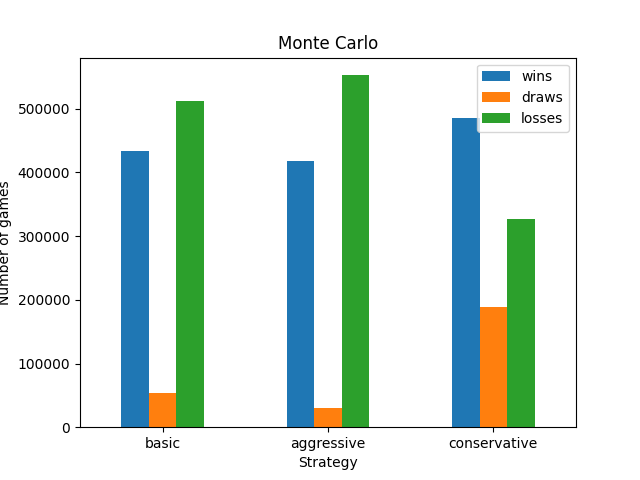
\includegraphics[width=0.5\textwidth]{src/mc.png}\\

Scalability is the ability of a parallel algorithm to efficiently utilize additional cores. The parallel algorithm is scalable because it achieves a speedup close to the theoretical speedup, indicating that it scales well with the number of cores used. The parallel algorithm is also efficient because it achieves a speedup of 4.22 for 10,000,000 trials, which is close to the theoretical speedup of 8.00. This indicates that the parallel algorithm is efficient and scales well with the number of cores used.

The graph below represents the scalability of the parallel algorithm. The graph shows that the speedup increases as the number of trials increases, indicating that the parallel algorithm scales well with the number of trials. The graph also shows that the speedup increases as the number of cores increases, indicating that the parallel algorithm scales well with the number of cores.\\
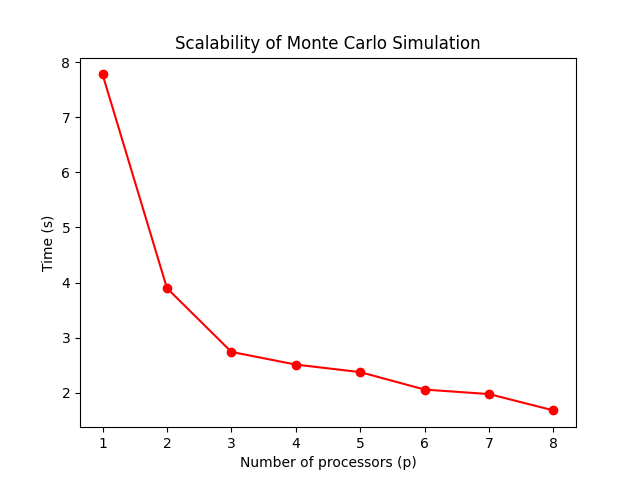
\includegraphics[width=0.5\textwidth]{src/mc_scale.png}

\section{Strategy Results}
The results from the optimal strategy are shown in bar charts below. The data is categorized in three ways: Wins, Draws, and Losses.
A win is when the player's hand is closer to 21 than the dealer's hand, a draw is when the player's hand is equal to the dealer's hand, and a loss is when the player's hand is further from 21 than the dealer's hand.\\
It is worth noting, that in the case of a draw, the player does not lose any money, but also does not gain any money. Therefore, draws are an important factor to consider, because if the sum of draws and wins are greater than losses. Then the strategy performs well.

\subsection{Basic Strategy}
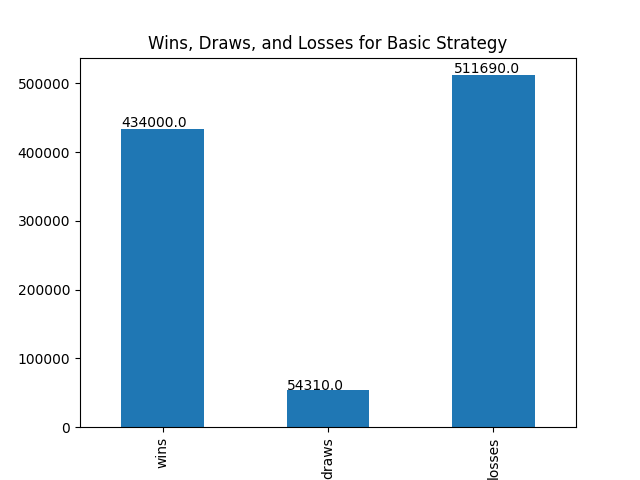
\includegraphics[width=0.5\textwidth]{src/basic.png}\\
As indicated by the bar chart, the basic strategy did not perform as well as the other two strategies. The basic strategy had the lowest number of wins, median number of draws and losses. This indicates that the basic strategy is not very effective at winning games of blackjack.

\subsection{Aggressive Strategy}
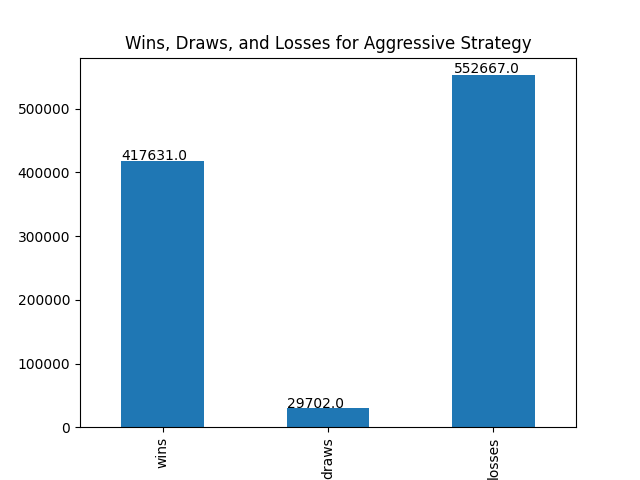
\includegraphics[width=0.5\textwidth]{src/aggressive.png}\\
The bar chart indicates that the aggressive strategy is the worst performing strategy. The aggressive strategy had the lowest number of wins and draws, with the highest number of losses. This indicates that the aggressive strategy is not very effective at winning games of blackjack.
This is likely due to the fact that the aggressive strategy is too risky, and therefore the player is more likely to bust.

\subsection{Conservative Strategy}
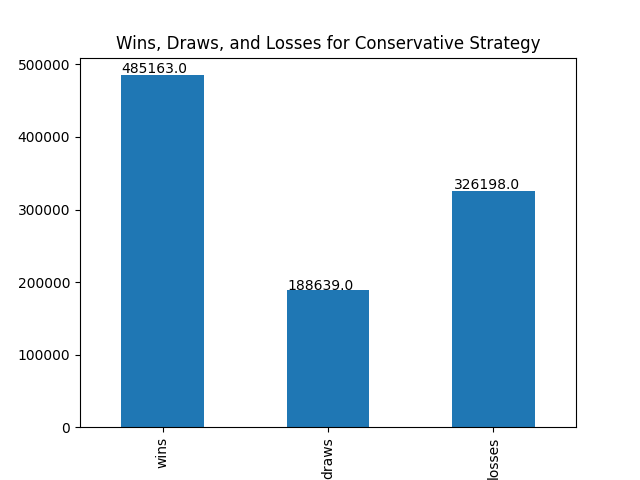
\includegraphics[width=0.5\textwidth]{src/conservative.png}\\
The final results show that this strategy is the best performing strategy. The conservative strategy had the highest number of wins and draws, with the lowest number of losses. This indicates that the conservative strategy is very effective at winning games of blackjack.
Since the number of draws is high, this indicates that the player is not taking too many risks, and is therefore not busting often.
This is profitable because the player is not losing money, and is also winning money.


\section{Conclusion}

Our exploration of Monte Carlo simulations for evaluating blackjack strategies through the lens of parallel computing has yielded significant findings. Our results confirm that parallelization is a powerful tool for improving the performance of Monte Carlo simulations. With OpenMP, we were able to significantly speed up computations, enabling a more efficient evaluation of blackjack strategies.

The choice of parallelization library is crucial to performance. OpenMP, with its shared-memory parallelism, is suitable for smaller scale computations, while MPI, with its distributed-memory parallelism, is apt for larger scale computations. It is noteworthy that despite the scale, both libraries provided substantial improvement in performance.

By implementing a parallel algorithm for the Monte Carlo simulations, we leveraged the full potential of modern multi-core processors. The use of OpenMP's parallel for loop construct allowed us to distribute the iterations across multiple threads, resulting in a substantial reduction in computation time. The application of several optimization techniques, such as reducing false sharing, loop scheduling, and nested parallelism, further enhanced the performance of our parallel algorithm.

In terms of blackjack strategies, the conservative strategy proved to be the most successful. Despite having the highest number of draws, the sum of wins and draws was higher than losses, indicating its effectiveness. This strategy played cautiously to avoid busting and relied on the dealer to bust, a tactic that proved to be profitable.

The parallel algorithm's scalability was demonstrated as it achieved a speedup close to the theoretical speedup, indicating that it efficiently utilized the increased number of cores. Its efficiency was further demonstrated by its performance, achieving a speedup of 4.22 for 10,000,000 trials, close to the theoretical speedup of 8.00.

In summary, our study confirms that parallel computing can significantly enhance the performance of Monte Carlo simulations for blackjack. With careful algorithm design and an appropriate choice of parallelization library, one can effectively analyze various blackjack strategies. While our research focused on blackjack, the methods and findings can be extended to other areas where Monte Carlo simulations are used, expanding the scope of this study beyond the realm of card games.

\end{document}


% Speedup for 1e7 trials = 8.06/1.91 = 4.22


